% -*- mode: latex; mode: auto-fill; coding: utf-8; -*-

The Total Lagrangian Explicit Dynamics solving technique (described in
section \ref{sec:tled_solver}), used to solve the finite element
equations is highly suited for parallel execution. So to
get optimal performance when implementing this technique, we need to
implement it for a parallel architecture.
%
The range of parallel technologies and platforms to choose from is
large, ranging from cluster farms, grid computers, graphics cards to
multi-cored central processing units (CPUs).
%
Motivated by the surgical scenario, and the request from densists to
use the simulator in educational training, we have chosen a hardware
platform, which is commonly available, inexpensive, and does not require
a large storage facility.
%
Two different platforms and accompanying APIs have been discussed, both
available as consumer products and affordable.
%
The first candidate was the Cell architecture, which
is commonly available in Sony's PlayStation 3. The PlayStation 3 is
suited for this kind of development because it allows custom installation of
an alternative operating system like Linux, and because both an API and
programming tools are freely available for Linux.
%
The second platform is an ordinary PC with a high performance graphics
card. Graphics cards nowadays are relatively powerful when considering
the computational power contra price.
%
We have chosen to base our implementation on multi-cored graphics
cards as this is a widely spread technology, and because we find the
provided programming abstractions and tools well suited for rapid
prototype development.
%

\section{Programming a Graphics Card}
The processing unit on a graphics card is called the graphics
processing unit (GPU), and general purpose programming of the GPU is
called GPGPU programming.
%
GPGPU programming has been done for quite a while now. The beginning was
a sort of misuse of the original APIs for the GPU. Programmers wrote
their applications in shader languages, which originally were intended
for producing graphical effects as part of the visualization.
%
As GPGPU programming has spread, new initiatives towards making a
general GPGPU API, like for example CUDA, has started to surface.
%
% By the time we started this thesis a vendor independent GPGPU
% programming language was not released. To the best of our knowledge
% the only option at that time was to implement the simulator in a low
% level shader language like GLSL if we wanted a hardware independent
% implementation. Since then the hardware independent programming
% language OpenCL has been introduced.
%
% The best thing would be to chose an environment which insured hardware
% independence across different hardware vendor's graphics cards. At the
% time we started our thesis this could only be done by writing the
% code in shader language. But writing programs in a low level shader
% programming language, like GLSL, which originally was not
% intended for GPGPU programming, is time consuming and not suitable for
% problems like our simulator.
%
We have chosen the CUDA programming language
developed by NVIDIA. This programming API has a higher level of
abstraction, it comes with useful libraries and is easy to use. The
drawback is that it is hardware dependent, and can therefore only be
used with NVIDIA graphics cards.
%   which at the same time provides better control over the
% actual hardware which makes it.

\layoutnewpage

% downwards copied from aotuflow report
\section{Basic Description of CUDA}
The Compute Unified Device Architecture (CUDA) is an
extension to the C programming language, which enables the programmer
to use the NVIDIA GPUs for GPGPU programming (this only apply for
NVIDIA 8000 or newer GPUs).
%
The extension includes special syntax, allowing programmers to
explicitly determine which parts of the program that is going to be
executed on the device. 
%
In CUDA terminology a \defit{host} refers to the CPU with access to the main
memory, and the \defit{device} refers to a specific graphic card with access
to the available memory, known as \defit{global memory}, on the graphics card.
%
% that a function is to be executed on the GPU. A function
% executed this way is called a \defit{kernel} \{tic}{Check
%   terminology used here}. 
%
In CUDA the kernels are launched with parameters defining the
\defit{block} and \defit{grid} size. Threads are executed in
blocks which are wrapped in a grid,
% upwards copied from aotuflow report
as illustrated in figure \vref{fig:cuda-grid}.

\begin{figure}
  \centering
  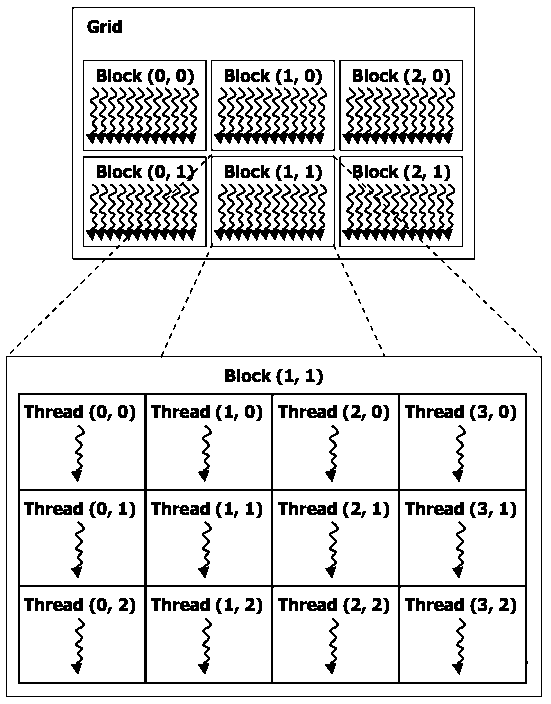
\includegraphics[width=7cm]{./images/parallel_execution_cuda_grid.png}
\caption{Illustration of the CUDA grid, block, and thread
  abstractions. $\ddagger$}
\label{fig:cuda-grid}
\end{figure}

% downwards copied from aotuflow report
When a kernel is launched the grid is set for execution. When
executing the grid each block is scheduled one by one and 16 threads
from the block are executed simultaneously by the hardware in what is
known as a \defit{half warp}. The execution order of the blocks and
warps is non-deterministic and can be different every time the program
is executed. The execution and scheduling of threads is performed by
the device. 
%are done in
%hardware, which runs very fast.
%
The extension also includes special keywords which can be used inside
kernels to access the dimensions and identifiers of the thread, block
and grid.
% upwards copied from aotuflow report

\section{Our Implementation}
The CUDA technology allows code to be executed in parallel. The
parallel execution used here is based on the \defit{Single Instruction,
Multiple Thread (SIMT)} technique used to achieve data level parallelism. 
This technique is closely related to the wide known
\defit{Single Instruction, Multiple Data (SIMD)}.
It basically means that multiple threads are executing the
same program (same set of instructions) in parallel but with different
data.
%
% Parallel execution here referes to that the GPU have 
% multiple processing units, and can execute the same program with
% different data at the same time. The technology does not allow to run
% programs on the CPU and GPU at the same time. 
When executing parts of the program in parallel we use blocking calls
to start kernels on the GPU, this means that either the host or
device is active. Switching from the host to the device, must be done
explicitly in the code by executing a kernel. The host and the
device have separate memory spaces. If data needs processing on both
the host and the device it needs to be copied from one memory space to
the other. \\
%
% is needed from the other
% parties memory this must also be copied manually. The memory connected
% the the CPU is call the \defit{main memory} and for the GPU it is
% called \defit{global memory}. \newline
%

We will now elaborate on how the finite element system equations are
solved by element-wise computations and how the individual solutions
are assembled by the end of each iteration.
%The following will try to make clear how the TLED solver works when it
%solves the system. 
Consider the element equation
\eqref{eq:matrix-equation-for-element-a} for one tetrahedron, as
explained in section \vref{sec:example-of-two-tetrahedrons}. The
equation is repeated below:

\begin{equation*}
F^a = K^a U^a
\qquad \Leftrightarrow \qquad
\begin{bmatrix}
f^1 \\
f^2 \\
f^3 \\
f^4
\end{bmatrix}
=
\begin{bmatrix}
K^a_{11} & K^a_{12} & K^a_{13} & K^a_{14} \\
K^a_{21} & K^a_{22} & K^a_{23} & K^a_{24} \\
K^a_{31} & K^a_{32} & K^a_{33} & K^a_{34} \\
K^a_{41} & K^a_{42} & K^a_{43} & K^a_{44}
\end{bmatrix}
\begin{bmatrix}
u^1 \\
u^2 \\
u^3 \\
u^4
\end{bmatrix}
\end{equation*}

These equations can be easily computed in parallel for each element.
It is when elements are connected and hereby interacting it gets
more complex. When elements are connected they share nodal points. The
shared nodal points can be seen explicit by looking at the final
system equation. Consider the example from section
\vref{sec:example-of-two-tetrahedrons} again, here we directly see each
element's contribution to the shared nodal variables. They are seen as
weights ($K_{ij}^e$) added together in the matrix. The system matrix
from equation \eqref{eq:system-stiffness-matrix} in the example is
repeated below for convenience:

\begin{equation*}
K = K^A + K^B =
\begin{bmatrix}
K^a_{11} & K^a_{12} & K^a_{13} & K^a_{14} & 0\\

K^a_{21} & K^a_{22} + K^b_{11} & K^a_{23} + K^b_{12} & K^a_{24} +
K^b_{13} & K^b_{14}\\

K^a_{31} & K^a_{32} + K^b_{21} & K^a_{33} + K^b_{22} & K^a_{34} +
K^b_{23} & K^b_{24}\\

K^a_{41} & K^a_{42} + K^b_{31} & K^a_{43} + K^b_{32} & K^a_{44} +
K^b_{33} & K^b_{34}\\

0 & K^b_{41} & K^b_{42} & K^b_{43} & K^b_{44}
\end{bmatrix}
\end{equation*}

Since the element equations are added together we can skip the
construction of the system stiffness matrix, and instead add the
individual nodal contributions from each element. This is
the approach used by the TLED solver which can be summarized as:
%
% in this kernel all element stiffness matrix calculations are done, the
% result being weights in the element stiffness matrix (this is actual
% forces).
%
% afterwards a kernel called .. visual... is called, this kernel is run
% per node. the kernel sums all the displacement contributions for each
% element, so only one displacement vector remains at each vertex.
%
%our main physics module is implemented. 
%Our implementation does this as follows:

\begin{itemize}
\item The external nodal forces are applied by the user interaction
  module and processed by the finite element solver. This data is located in the
  main memory and copied to global device memory as the first step.
\item We then start the main solver kernel (TLED solver) called
  \code{calculateForces\_k}. This kernel is executed for each
  element, and performs all calculations as explained in section
  \vref{sec:tled_solver}.
  The resulting list of nodal force contributions are saved in global memory.
  Furthermore this kernel solves the eigenproblem for each element, and
  detects if the material dependent fracturing limit has been
  exceeded. If so it raises a flag.
\item The nodal force contributions are now being added together for each
  node to determine the resulting force and displacement. This kernel
  is named \code{updateDisplacements\_k}. The resulting displacements
  are stored in global memory, one displacement vector for each node.
\item The final kernel is named (\code{updateBodyMesh\_k}) and it updates the
  surface and body mesh by adding the displacement vector to the
  initial position for each node. Updating the global nodal positions
  is only done for visualization purposes. Due to the small
  simulation time step performed in each iteration we solve the system
  equations multiple times in between the visualizations. 
\end{itemize}

The finite element solver is executed every iteration of the main-loop, but 
the visualization of the surface, does not need to be updated this
often. The visualization is set at approximately 30 frames per second
(FPS), guaranteeing fluent motion of the visual animations.
%
The visualization of the surface is done via the CUDA OpenGL
interoperability API. This API allows OpenGL to access the memory used
by the CUDA programs and directly visualizes it without the need of
copying the data back and forth between main and global memory.

\subsection{Execution Time}
\label{sec:exection_time}
To get an overview of how time consuming the different kernels are, we
have made time measurements of each kernel executed.
The test was performed on the laptop described in appendix
\vref{sec:test-machines-latop} with version 1.2 of the CUDA Visual
Profiler, using the tooth mesh described in appendix
\appref{sec:test-data-tooth}. Table \vref{table:cuda-progiler-data} shows
the result from the profiler.

% The data shows execution of the simulation
% from start up and running some iterations, the \# calls column is how
% many times the kernel have been executed.

\begin{table}
  \centering
  \begin{tabular}{| l | r | r | r |}
    \hline
    kernel name & \# calls & GPU microseconds & \% GPU time \\
    \hline
calculateForces\_k                 & 52325 & 10968700 & 65.45 \\
updateDisplacements\_k             & 52325 &  2893260 & 17.26 \\
testCollision\_k                   & 54417 &  1605060 &  9.57 \\
memcopy                                       & 25115 &      966304 &  5.76 \\
applyForceToIntersectingNodes\_k              & 54417 &      131965 &  0.78 \\
constrainIntersectingPoints\_k                & 54417 &      125802 &  0.75 \\
updateBodyMesh\_k                             &  2093 &       67304 &  0.40 \\
precalculateShapeFunctionDerivatives\_kernel  &     1 &      22 &  0.00 \\
loadArrayIntoVBO\_k                           &     8 &      18 &  0.00 \\
applyTransformation\_k                        &     2 &       9 &  0.00 \\
precalculateABC\_kernel                       &     1 &       6 &  0.00 \\
    \hline
  \end{tabular}
  \caption{Profiling results.}
  \label{table:cuda-progiler-data}
\end{table}

To get an visual overview of the percentages, the following diagram
illustrated kernels that is part of one iteration, and not
pre-computational kernels.

\begin{figure}
  \centering
  \subfloat[Diagram.]{
    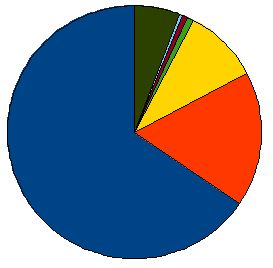
\includegraphics[width=5cm]{./images/parallel_execution_cuda_pie_diagram.png}
    \label{fig:cuda-pie-diagram}
  }
  \subfloat[Information.]{
    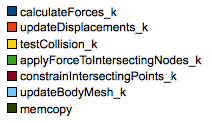
\includegraphics[width=5cm]{./images/parallel_execution_cuda_pie_info.png}
    \label{fig:cuda-pie-info}
  }
  \caption{GPU time spent on the individual kernels.}
  \label{fig:cuda-pie}
\end{figure}

About $2/3$ of the computational resources on the device is spent on
processing the finite element solver which is not surprising considering the
complexity compared to the other tasks.
%
% As illustrated the resources he physics module takes
%  about $2/3$ of the
% over all execution time.
% Here we clearly see that the physics module takes about $2/3$ of the
% over all execution time.\{cpvc}{describe the kernels which are not mentioned}

\section{Optimizing Performance}
% downwards copied from aotuflow report
To get optimal performance from the device through CUDA we need to
overcome the memory latency limitation imposed. The memory bus on
the graphics cards has a high bandwidth but also a large latency when
fetching from the global memory. When programming in CUDA one needs to be
aware of the fact that memory fetching must be done in correspondence
to the alignment and coalescing rules as described in
\citeabook{book:cuda-pg}. The alignment and coalescing constraints
allow the GPU to effectively hide the memory latency.
% upwards copied from aotuflow report
%
We want the simulation to run in real-time, therefore all code inside
the main-loop has been optimized for performance in relation to these
guidelines As most of this code is executed on the device, the main
concerns are the memory latency as described.

% \subsection{Aligned Memory}
% We must insure that CUDA makes the minimum number of memory
% transaction when the code is running. By using simple types, like
% \code{int} and \code{float} and the extra types provided by CUDA like
% \code{float2}, \code{float4}, etc., the memory is automatically
% aligned to 8 and 16 bit boundaries. This insures that a minimum number
% of memory transactions are needed when fetching variables.

\subsection{Using float4 Instead of float3}
CUDA devices are capable of reading 4-byte, 8-byte or 16-byte words,
corresponding to 32-bit, 64-bit, and 128-bit operations,
from global memory into thread registers when executing threads
\citebook{page~81}{book:cuda-pg}.
%
In our simulation we often use three consecutive floats. For example when
representing vectors in space, like global coordinates, displacements,
etc. If we represented this by three \code{float} variables, CUDA would
generate two memory operations to fetch the memory, one 32-bit and one
64-bit. Instead we use one \code{float4}, which corresponds to a
single 128-bit memory operation, resulting in faster memory
fetching. The increased performance is at the expense of increased
memory consumption.

\subsection{Coalesced Memory Access}
Global memory bandwidth is used most efficiently when the simultaneous
memory accesses by threads in a half-warp, can be coalesced into a
single memory transaction of 32, 64 or 128 bytes
\citebook{page~82}{book:cuda-pg}.
%
This means that if the threads are using memory cells located
next to each other in an array the memory for all the threads
can be fetched in one transaction or block copied of the memory.
%
To facilitate this we use the same memory allocation scheme as 
\citebook{page~55-56}{Rasmusson2008}. Instead of allocating
tetrahedral elements side by side, we use arrays of individual
variables related to all tetrahedra. This means that arrays are
allocated for storing all densities, all masses, all nodal indices
etc.

%Compute Capability 1.0 and 1.1 compared to 1.2 and Higher, page 82-83.

